\documentclass[notheorems,serif,table,compress]{beamer}  %dvipdfm选项是关键,否则编译统统通不过
%%------------------------常用宏包------------------------
%%注意, beamer 会默认使用下列宏包: amsthm, graphicx, hyperref, color, xcolor, 等等
\usepackage{fontspec,xunicode,xltxtra}  % for XeTeX
\usepackage{verbatim}
\usepackage{mathabx}
\usepackage{latexsym}
\usepackage{amsfonts,amssymb}
\usepackage{styles/iplouclistings}
\usepackage{fancybox}
\usepackage{colortbl}
\usepackage{tcolorbox}
%\usepackage[T1]{fontenc}
%\usepackage{bookman}
\usepackage{subfigure}
\usepackage{hyperref}
\usepackage{listings}
\usepackage{animate}
\usepackage[absolute,overlay]{textpos}
\usepackage{graphicx}
\usepackage{tikz}
\usepackage[americaninductors,europeanresistors]{circuitikz}
\usepackage{tikz}
\usepackage{fancybox}     %% 定义zhushadow时用到
\usepackage{pifont} %ding用到
\newsavebox{\mysaveboxOne}  %%为了在only中使用lstlisting
\newsavebox{\mysaveboxTwo}
\newsavebox{\mysaveboxThree}
\newsavebox{\mysaveboxFour}
\newsavebox{\mysaveboxFive}
\newsavebox{\mysaveboxSix}
\newsavebox{\mysaveboxSeven}
\newcommand\zhushadow[2][purple]{\hskip5pt\shadowbox{\color{#1}\small\kai #2\vspace{3mm}}}

%%------------------------ThemeColorFont------------------------
%% Presentation Themes
% \usetheme[<options>]{<name list>}
%\usetheme{Madrid}
\usetheme{Berkeley}
%% Inner Themes双精度计算
% \useinnertheme[<options>]{<name>}
%% Outer Themes
% \useoutertheme[<options>]{<name>}
%\useoutertheme{miniframes} 
%% Color Themes 
%\usecolortheme[<options>]{<name list>}
%% Font Themes
\usefonttheme{serif}
\setbeamertemplate{background canvas}[vertical shading][bottom=white,top=structure.fg!7] %%背景色, 上25%的蓝, 过渡到下白.
\setbeamertemplate{theorems}[numbered]
\setbeamertemplate{navigation symbols}{}   %% 去掉页面下方默认的导航条.
\usepackage{styles/zhfontcfg}
%\setsansfont[Mapping=tex-text]{文泉驿正黑}  %% 需要fontspec宏包
     %如果装了Adobe Acrobat,可在font.conf中配置Adobe字体的路径以使用其中文字体
     %也可直接使用系统中的中文字体如SimSun,SimHei,微软雅黑 等
     %原来beamer用的字体是sans family;注意Mapping的大小写,不能写错
     %设置字体时也可以直接用字体名,以下三种方式等同:
     %\setromanfont[BoldFont={黑体}]{宋体}
     %\setromanfont[BoldFont={SimHei}]{SimSun}
     %\setromanfont[BoldFont={"[simhei.ttf]"}]{"[simsun.ttc]"}
%%------------------------MISC------------------------
\graphicspath{{figures/}}         %% 图片路径. 本文的图片都放在这个文件夹里了.
%%------------------------listing------------------------
%\lstset{language=[LaTeX]TeX,Python}
%%------------------------正文------------------------
\begin{document}
\XeTeXlinebreaklocale "zh"         % 表示用中文的断行
\XeTeXlinebreakskip = 0pt plus 1pt % 多一点调整的空间
%%----------------------------------------------------------
%% This is only inserted into the PDF information catalog. Can be left
%% out.
%%%
%% Delete this, if you do not want the table of contents to pop up at
%% the beginning of each subsection:
%\AtBeginSection[]{                              % 在每个Section前都会加入的Frame
%  \frame<handout:0>{
%    \frametitle{Contents}\small
%    \tableofcontents[current,currentsubsection]
%  }
%}
%
%\AtBeginSubsection[]                            % 在每个子段落之前
%{
%  \frame<handout:0>                             % handout:0 表示只在手稿中出现
%  {
%    \frametitle{Contents}\small
%    \tableofcontents[current,currentsubsection] % 显示在目录中加亮的当前章节
%  }
%}

\setbeamertemplate{caption}{\raggedright\insertcaption\par}

%%----------------------------------------------------------
\logo{
\includegraphics[scale=0.13]{ouclogo.png}}
\title{Edge-based Segmentation}
%\subtitle{Bottom-Up Saliency Detection Model Based on Human Visual Sensitivity and Amplitude Spectrum}
\subtitle{基于边缘的图像分割}
\author[]{\textcolor{olive}{ZhaoHaiwei DaiJialun WangRuchen}}
\institute[CVBIOUC]
{
\small\textcolor{violet}{CVBIOUC\\
%Ocean University of China\\
\url{http://vision.ouc.edu.cn/~zhenghaiyong}}
}
%\date[]{}
%\titlegraphic{
%
\includegraphics[height=1.0cm]{ouc-logo.jpg}}
\frame{ \titlepage }
%%----------------------------------------------------------
%\section*{Contents}
\frame{\frametitle{Contents}\tableofcontents}
%%----------------------------------------------------------
\def\hilite<#1>{\temporal<#1>{\color{blue!15}}{\color{black}}{\color{black}}}
\newcommand{\shadow}[2][purple]{\hskip5pt\shadowbox{\color{#1}\small \kai #2\vspace{3mm}}}
\newcommand{\colorrbox}[2][purple]{\doublebox{\color{#1}\small \kai#2}}

%============================================================================

\section{Introduction}

%==========================================================================


\begin{frame}[fragile]
\frametitle{What?}
    \begin{figure}
    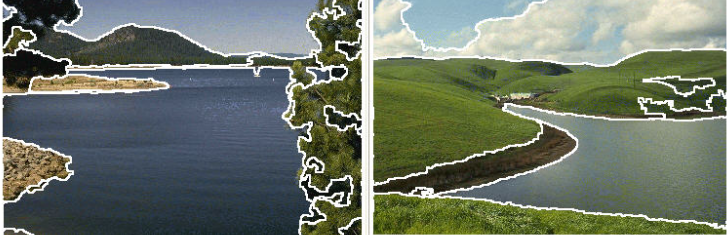
\includegraphics[width=0.8\linewidth]{edgeseg.png} 
    \end{figure}
\end{frame}


\subsection{Edge \& Boundary}

\begin{frame}
\frametitle{Edge \& Boundary}
    \begin{tcolorbox}[colback=red!5,colframe=blue!75!black]
        \begin{figure}
            \begin{minipage}[t]{0.3\linewidth}
            \centering
            \caption{original image}
            
\includegraphics[width=1\linewidth]{src.png} 
            \end{minipage}
            \begin{minipage}[t]{0.3\linewidth}
            \centering
            \caption{edge}
            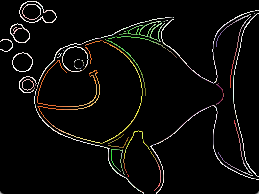
\includegraphics[width=1\linewidth]{edge.png} 
            \end{minipage}
            \begin{minipage}[t]{0.3\linewidth}
            \centering
            \caption{boundary}
            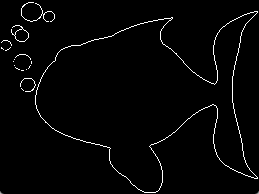
\includegraphics[width=1\linewidth]{bounary.png} 
            \end{minipage}
        \end{figure}
    \end{tcolorbox}
~~~~~The edge of object may be not a boundary, the boundary may also be not edge.
\end{frame}
 
 
\subsection{Problems}

\begin{frame}
\frametitle{Problems}
Edge detection is a simple and fast technique used in segmentation methods. However, there also are some problems:
    \begin{itemize}
        \item {\color{blue}{\textbf{Noise}} and {\textbf{background}} affect the accurate of edge detection.}
        \item Edges are the sign of lack of continuity, and ending.
    \end{itemize}
    \begin{figure}
        \begin{minipage}[t]{0.4\linewidth}
        \centering
        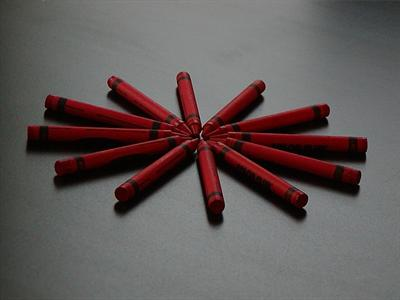
\includegraphics[width=1\linewidth]{0_0_284.jpg} 
        \end{minipage}
        \begin{minipage}[t]{0.4\linewidth}
        \centering
        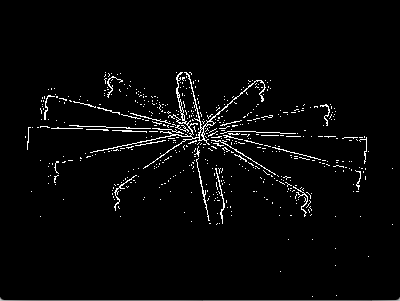
\includegraphics[width=1\linewidth]{noise.png} 
        \end{minipage}
    \end{figure}
\end{frame}


\subsection{Steps in Edge Detection}

\begin{frame}
\frametitle{Steps in Edge Detection}
    \begin{enumerate}
        \item {\color{blue}Filtering:} Filtering to reduce noise results in a loss of edge strength.
        \item {\color{blue}Enhancement:} In order to facilitate the detection of edges, it is essential to determine changes in intensity in the neighborhood of a point. 
        \item {\color{blue}Detection:} Find the zero crossing and peak value to detect edge.
    \end{enumerate}
\end{frame}

\begin{frame}
\frametitle{Problems}
Edge detection is a simple and fast technique used in segmentation methods. However, there also are some problems:
    \begin{itemize}
        \item Noise and background affect the accurate of edge detection.
        \item {\color{blue}Edges are the sign of {\textbf{lack of continuity}}, and ending.}
    \end{itemize}
    \begin{figure}
        \begin{minipage}[t]{0.4\linewidth}
        \centering
        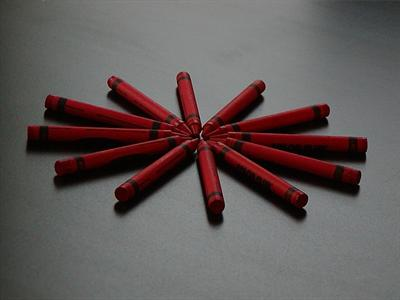
\includegraphics[width=1\linewidth]{0_0_284.jpg} 
        \end{minipage}
        \begin{minipage}[t]{0.4\linewidth}
        \centering
        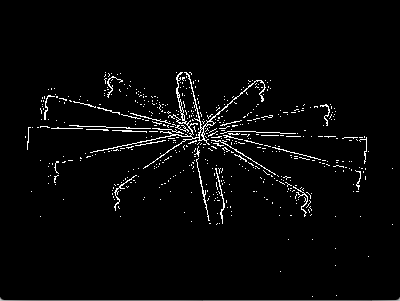
\includegraphics[width=1\linewidth]{noise.png} 
        \end{minipage}
    \end{figure}
\end{frame}


\subsection{Steps in Image Segmentation}

\begin{frame}
\frametitle{Step in Image Segmentation}
    \begin{figure}
    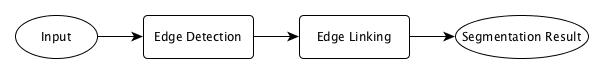
\includegraphics[width=1\linewidth]{liucheng.jpg} 
    \end{figure}
\end{frame}



%============================================================================

\section{Edge Detection}

%============================================================================

\begin{frame}
\frametitle{Edge Detection}
Three edge types and definitions:
    \begin{itemize}
        \item Step edge
        \item Ramp edge
        \item Roof edge
    \end{itemize}
    \begin{figure}
    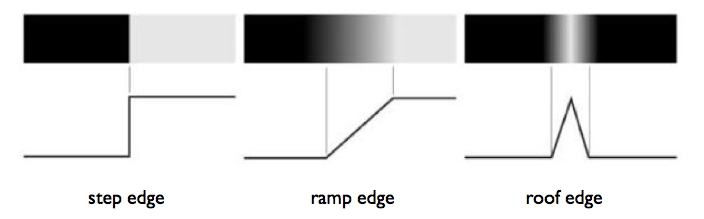
\includegraphics[width=0.9\linewidth]{bian.png} 
    \end{figure}
\end{frame}

\begin{frame}
\frametitle{Edge Detection}
    \begin{figure}
    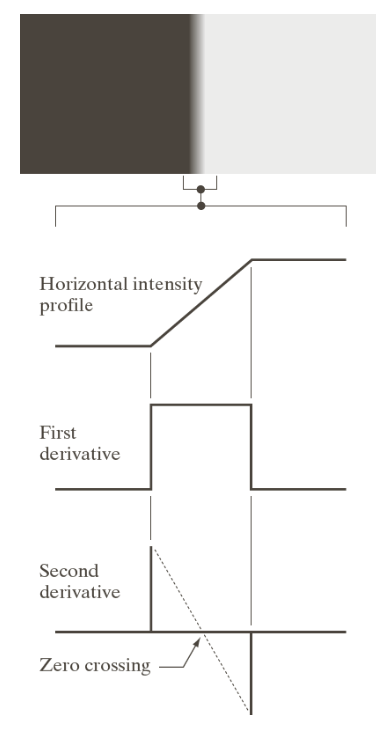
\includegraphics[width=0.35\linewidth]{jiance.png} 
    \end{figure}
\end{frame}


\begin{frame}
\frametitle{Edge Detection Techniques\footnote{Rafael C. Gonzalez \textit{et al.}, ``Digital Image Processing'', Publishing House of Electronics Industry, 2011. }}
    \begin{itemize}
        \item Roberts Edge Detection
        \item Sobel Edge Detection
        \item Prewitt Edge Detection\\
        $\dots$\newline
        
        \item Marr-Hildreth Edge Detection (LoG)
        \item Canny Edge Detection
    \end{itemize}
\end{frame}

\begin{frame}
\frametitle{Gradient}
The gradient $\bigtriangledown f$ of a function is: 
    \begin{displaymath}
        \bigtriangledown f = grad(f ~) = \left[\begin{array}{c}
    		          g_{x}  \\
    		          g_{y}  \\
    		         \end{array}\right]
        =\left[ \begin{array}{c}
    		          \frac{\partial f}{\partial x}  \\
    		          \frac{\partial f}{\partial y}  \\
    		         \end{array} \right]
    \end{displaymath}
The {\textbf{magnitude}} of the gradient is:
    \begin{displaymath}
        M(x,y)=mag(\bigtriangledown f ~) = \sqrt{g_{x}^{2}+g_{y}^{2}}
    \end{displaymath}
The {\textbf{direction}} of the greatest rate of change is:
    \begin{displaymath}
        \alpha (x,y)=arctan \left[ \frac{g_{x}}{g_{y}} \right]
    \end{displaymath}
\end{frame}


\subsection{Edge Detection Techniques}

\begin{frame}        
\frametitle{Edge Detection Techniques}
    \begin{figure}
    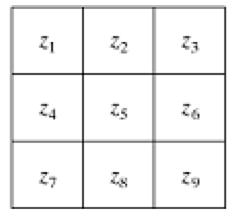
\includegraphics[width=0.2\linewidth]{mo.png} 
    \end{figure}
    \begin{itemize}
    \item Roberts Edge Detection
        \begin{figure}
        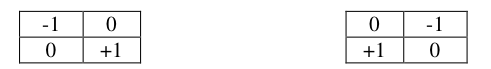
\includegraphics[width=0.8\linewidth]{roberts.png} 
        \end{figure}
    \end{itemize}
    \begin{displaymath}
    g_{x}= \frac{\partial f}{\partial x}=z_{9}-z_{5}
    \end{displaymath}
    \begin{displaymath}
    g_{y}= \frac{\partial f}{\partial y}=z_{8}-z_{6}
    \end{displaymath}
\end{frame}

\begin{frame}
\frametitle{Edge Detection Techniques}
    \begin{itemize}
        \item Sobel Edge Detection
            \begin{figure}
            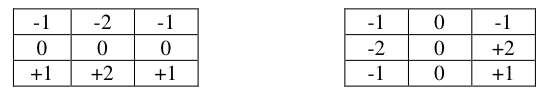
\includegraphics[width=0.8\linewidth]{sobel.png} 
            \end{figure}
            \begin{displaymath}
            g_{x}= \frac{\partial f}{\partial x}=(z_{7}+2z_{8}+z_{9})-(z_{1}+2z_{2}+z_{3})
            \end{displaymath}
            \begin{displaymath}
            g_{y}= \frac{\partial f}{\partial y}=(z_{3}+2z_{6}+z_{9})-(z_{1}+2z_{4}+z_{7})
            \end{displaymath}
        \item Prewitt Edge Detection
            \begin{figure}
            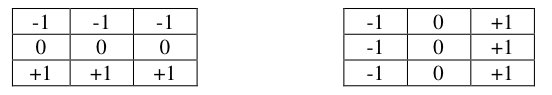
\includegraphics[width=0.8\linewidth]{prewitt.png} 
            \end{figure}
    \end{itemize}
\end{frame}


\subsection{Marr-Hildreth}

\begin{frame}
\frametitle{Marr-Hildreth Edge Detection (LoG)\footnote{Marr D, Hildreth E, ``Theory of Edge Detection'', Proc. of the Royal Society of London, 1980.}}
    \begin{columns}
        \begin{column}{0.55\linewidth}
            This method combines {\textbf{Gaussian filtering}} with the {\textbf{Laplacian}} for edge detection.\newline
            
            {\color{blue}Idea:}
            \begin{enumerate}
            \item {\color{blue}Gaussian filer} is used to swipe away noise from the image
            \item {\color{blue}Laplace operator}
            \item  Locate {\color{blue}zero crossings}
            \end{enumerate}
        \end{column}
        \begin{column}{0.45\linewidth}
            \centering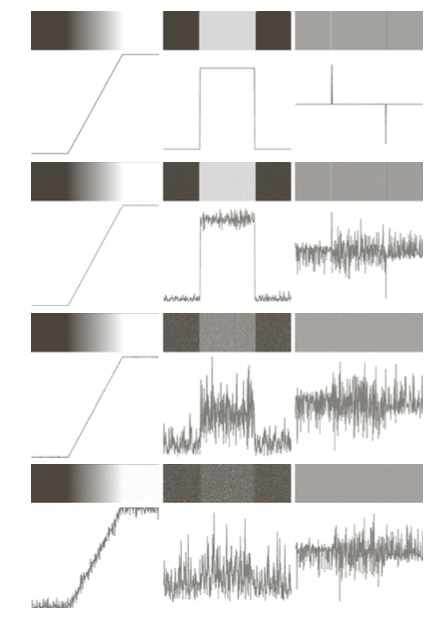
\includegraphics[width=1.5in]{erjie.png}
        \end{column}
    \end{columns}\vspace{1ex}
\end{frame}


\subsection{Canny Edge Detection}

\begin{frame}
\frametitle{Canny Edge Detection\footnote{Joun F. Canny, ``A Computational Approach To Edge Detection'', PAMI, 1986.}}
Canny is the best edge detection detector.\newline

    {\color{blue}Idea:}
    \begin{enumerate}
        \item Low error rate
        \item Edge points should be well localized
    \end{enumerate}
\end{frame}

\begin{frame}
\frametitle{Canny Edge Detection}
{\color{blue}Canny algorithm:}
    \begin{figure}
        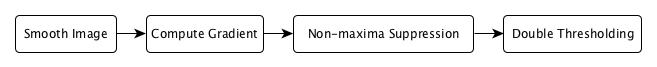
\includegraphics[width=1\linewidth]{cannyliu.jpg} 
    \end{figure}
    \begin{figure}
        \begin{minipage}[t]{0.22\linewidth}
            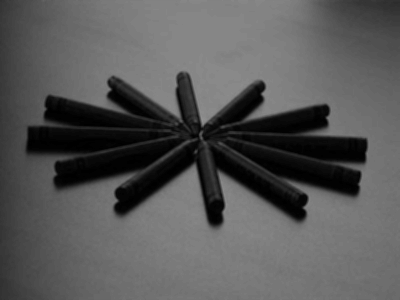
\includegraphics[width=1\linewidth]{gauSmooth.png} 
        \end{minipage}
        \begin{minipage}[t]{0.22\linewidth}
            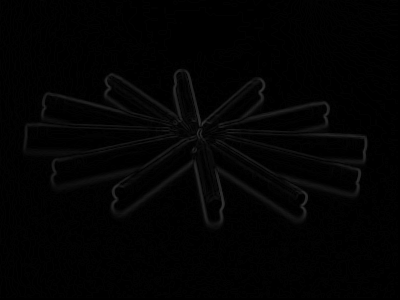
\includegraphics[width=1\linewidth]{gradResult.png} 
        \end{minipage}
        \begin{minipage}[t]{0.22\linewidth}
            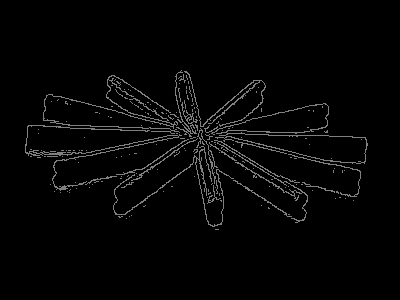
\includegraphics[width=1\linewidth]{nonResult.png} 
        \end{minipage}
        \begin{minipage}[t]{0.22\linewidth}
            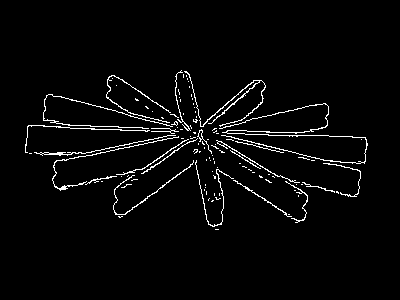
\includegraphics[width=1\linewidth]{cannyResult.png} 
        \end{minipage}
    \end{figure}
\end{frame}

\begin{frame}
\frametitle{Canny Edge Detection}
{\color{blue}Gauss Filter:}
    \begin{enumerate}
        \item Gaussian distribution
            \begin{columns}
            \begin{column}{0.55\linewidth}
              \begin{itemize}
                \item \emph{one dimension:}
                    \begin{displaymath}
                    G(x)=\frac {1}{\sqrt{2\pi}\sigma}e^{-\frac{x^{2}}{2\sigma^{2}}}
                    \end{displaymath}
                \item \emph{two dimension:}
                    \begin{displaymath}
                    G(x,y)=\frac {1}{2\pi \sigma^{2}}e^{-\frac{x^{2}+y^{2}}{2\sigma^{2}}}
                    \end{displaymath}
              \end{itemize}
            \end{column}
            \begin{column}{0.45\linewidth}
                \centering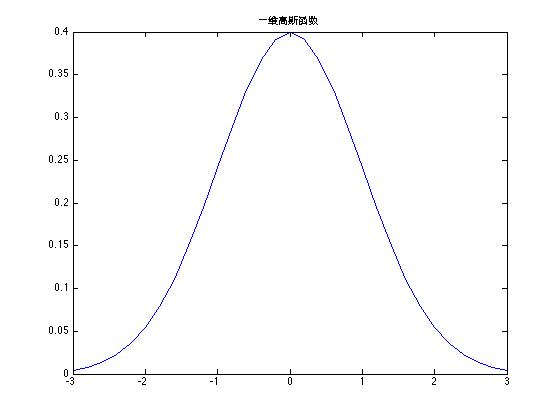
\includegraphics[width=0.6\linewidth]{gaoyi.jpg}
                
                \centering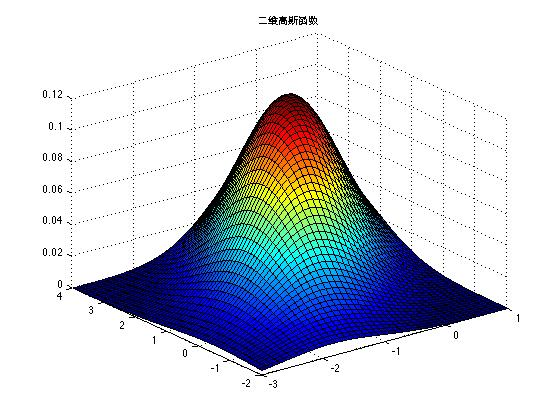
\includegraphics[width=0.6\linewidth]{gaoer.jpg} 
            \end{column}
            \end{columns}\vspace{1ex}
        \item Gaussian kernel
            \begin{figure}
            \centering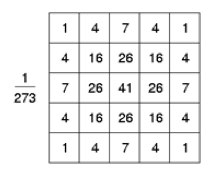
\includegraphics[width=0.2\linewidth]{gaosihe.png} 
            \end{figure}
    \end{enumerate}
\end{frame}

\begin{frame}
\frametitle{Canny Edge Detection}
{\color{blue}Compute Gradient:}
    \begin{displaymath}
    S_{x}=\left[ \begin{array}{cc}
    -1 & 1 \\
    -1 & 1 \\
    \end{array} \right],
    S_{y}=\left[ \begin{array}{cc}
    1 & 1 \\
    -1 & -1 \\
    \end{array} \right]
    \end{displaymath}
    \begin{figure}
        \begin{minipage}[t]{0.45\linewidth}
            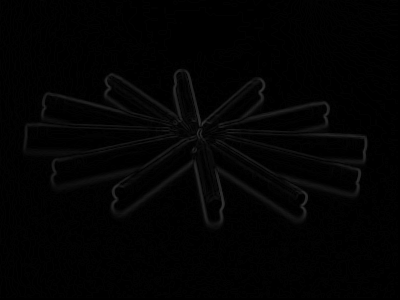
\includegraphics[width=1\linewidth]{gradResult.png} 
        \end{minipage}
        \begin{minipage}[t]{0.45\linewidth}
            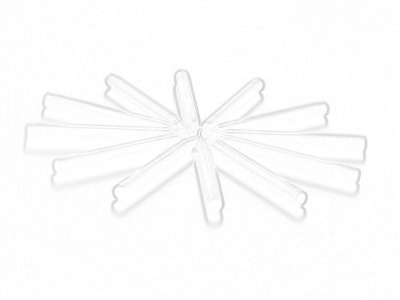
\includegraphics[width=1\linewidth]{not.png} 
        \end{minipage}
    \end{figure}
\end{frame}

\begin{frame}
\frametitle{Canny Edge Detection}
{\color{blue}Non-maxima Suppression (NMS):}
    \begin{itemize}
        \item Edges generated using gradient typically contain {\textbf{wide ridges}} around local maxima.
        \item Use non-maxima suppression to thin those ridges to find {\textbf{thin edges}} corresponding to local maxima.
    \end{itemize}
        \begin{figure}
        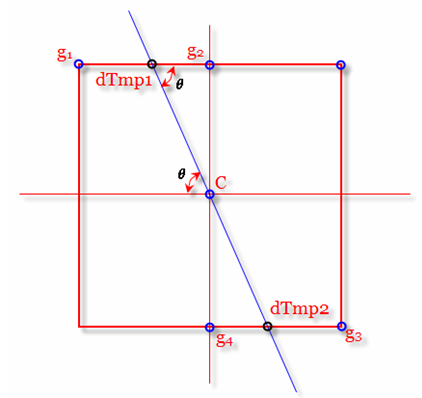
\includegraphics[width=0.4\linewidth]{nonmax.png} 
        \end{figure}
\end{frame}

\begin{frame}
\frametitle{Canny Edge Detection}
    \begin{figure}
    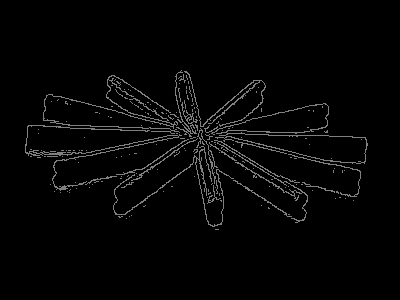
\includegraphics[width=0.7\linewidth]{nonResult.png} 
    \end{figure}
\end{frame}

\begin{frame}
\frametitle{Canny Edge Detection}
{\color{blue}Double thresholding:}
    \begin{itemize}
        \item {\color{blue}Problem:} The received image may still contain false edge points.
    \end{itemize}
        \begin{figure}
            \begin{minipage}[t]{0.35\linewidth}
                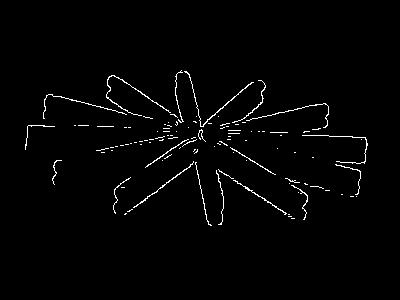
\includegraphics[width=1\linewidth]{height.png} 
            \end{minipage}
            \begin{minipage}[t]{0.35\linewidth}
                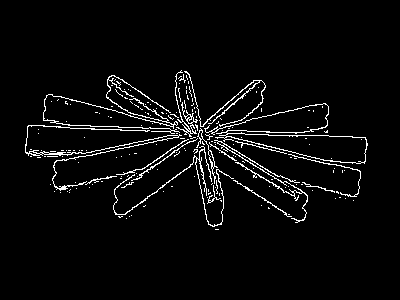
\includegraphics[width=1\linewidth]{low.png} 
            \end{minipage}
        \end{figure}
        \begin{figure}
            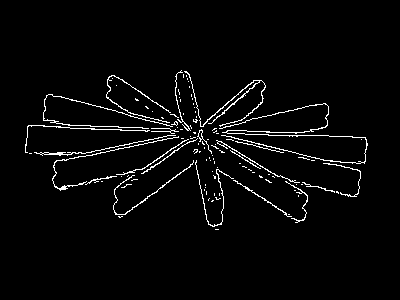
\includegraphics[width=0.35\linewidth]{cannyResult.png} 
        \end{figure}
\end{frame}

%============================================================================

\section{Edge Linking}

%============================================================================


\begin{frame}
\frametitle{Edge Linking}
    \begin{itemize}
        \item Edge Tracking
        \item Hough Transform
        \item Curve Fitting
        \item Dynamic Programming\\
        $\dots$
    \end{itemize}
\end{frame}
  
  
\subsection{Edge Tracking}

\begin{frame}
\frametitle{Edge Tracking}
{\color{blue}Idea:}
    \begin{itemize}
        \item Each point is linked to the adjacent if magnitude and direction of the gradient are {\textbf{similar}}.\newline
    \end{itemize}
    \begin{tcolorbox}[colback=red!5,colframe=blue!75!black]
    ~~~~$e(x,y)$ is magnitude of the gradient, $\theta(x,y)$ is the direction of the gradient, if two each points meet the following conditions:
        \begin{displaymath}
            \left\{ \begin{array}{ll}
            \mid e(x_{i},y_{i})-e(x_{j},y_{j}) \mid \leq E\\
            \mid \theta(x_{i},y_{i})-\theta(x_{j},y_{j}) \mid \leq A\\
            \mid e(x_{i},y_{i}) \mid , \mid e(x_{j},y_{j}) \mid > E
             \end{array} \right.
    \end{displaymath}
    \end{tcolorbox}
\end{frame}

\begin{comment}
\subsection{Curve Fitting}
\begin{frame}
\frametitle{Curve Fitting}
Starting from a set of edge points, segments of a polygonal line are iteratively added until all the points are close enough to a segment.
    \begin{figure}
        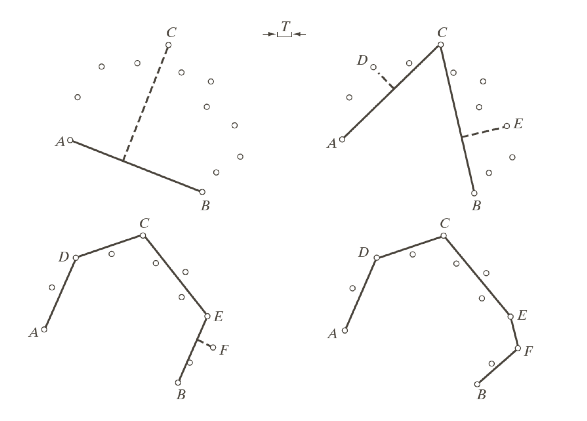
\includegraphics[width=0.6\linewidth]{duoni.png} 
    \end{figure}
\end{frame}
\end{comment}


\subsection{Hough Transform}

\begin{frame}
\frametitle{Hough Transform}
~~~~The Hough Transform can be used to detect {\color{blue}lines}, {\color{blue}circles} or other parametric curves.\newline

{\color{blue}Idea:}
    \begin{figure}[!ht]
        
\includegraphics[width=0.4\linewidth]{hough22.png}
    \end{figure}
\end{frame}

\begin{frame}
\frametitle{Hough Transform}
    \begin{figure}
        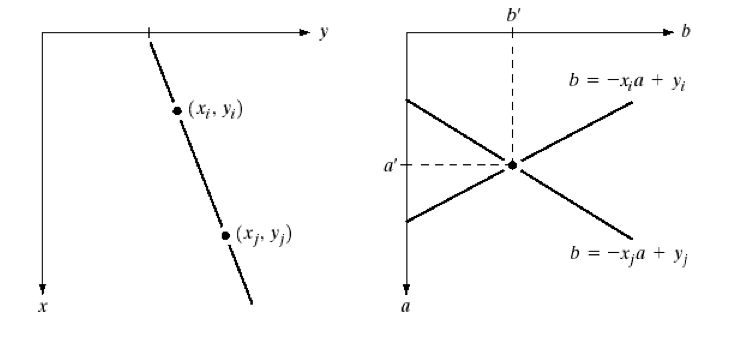
\includegraphics[width=0.8\linewidth]{hough.png} 
    \end{figure}
    \begin{displaymath}
        y=a^{'}x+b^{'}
        \qquad
        \left\{ \begin{array}{c}
        b = -x_{i}a+y_{i}\\
        b = -x_{j}a+y_{j}
        \end{array} \right.
    \end{displaymath}
\end{frame}

\begin{frame}
\frametitle{Hough Transform}
    \begin{figure}
        \begin{minipage}[t]{0.4\linewidth}
            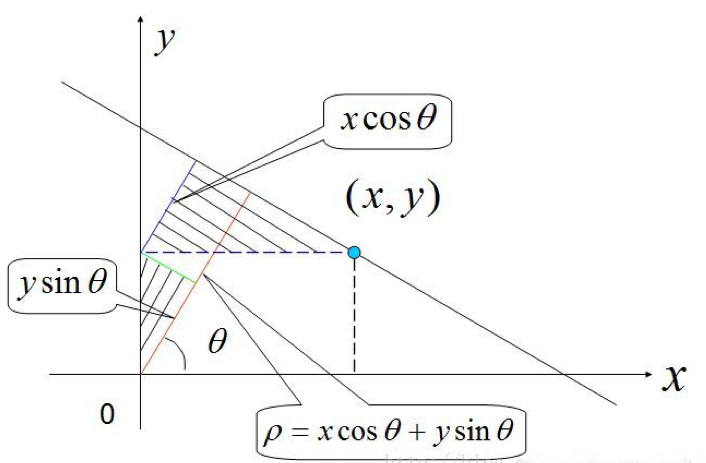
\includegraphics[width=1.5\linewidth]{hough1.png} 
        \end{minipage}
        \qquad 
        \qquad
        \quad
        \begin{minipage}[t]{0.4\linewidth}
            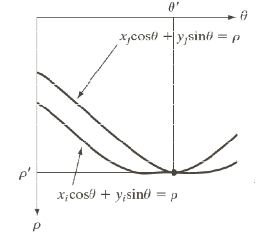
\includegraphics[width=1.05\linewidth]{hough3.png} 
        \end{minipage}
    \end{figure}
    \begin{displaymath}
        \left\{ \begin{array}{c}
        \rho^{'}=x_{i}cos\theta^{'} + y_{i}sin\theta^{'}\\
        \rho^{'}=x_{j}cos\theta^{'} + y_{j}sin\theta^{'}
        \end{array} \right.
         \qquad \Longrightarrow \qquad
        \left\{ \begin{array}{c}
        x_{i}cos\theta + y_{i}sin\theta= \rho\\
        x_{j}cos\theta + y_{j}sin\theta= \rho
        \end{array} \right.
    \end{displaymath}
\end{frame}

\begin{frame}
\frametitle{Hough Transform}
{\color{blue}Hough algorithm:}
    \begin{enumerate}
        \item Quantize the parameter space $(\rho,\theta)$. This quantized space is referred to as the {\textbf{accumulator cells}}.
        \item Count the number of times a line intersects a given cell.
        \item Lines can be found as peaks in this accumulator space.
            \begin{figure}
            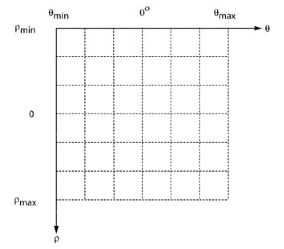
\includegraphics[width=0.5\linewidth]{hough4.png}
            \end{figure}
            \begin{displaymath}
            \rho=xcos\theta + ysin\theta
            \end{displaymath}
    \end{enumerate}
\end{frame}

\begin{frame}
\frametitle{Hough Transform}
{\color{blue}Circle:}
    \begin{figure}
        
\includegraphics[width=0.4\linewidth]{houghcir.png}
    \end{figure}
    \begin{displaymath}
        (x-a)^{2}+(y-b)^{2}=r
    \end{displaymath}
\end{frame}

\begin{frame}
    \begin{figure}
        \begin{minipage}[t]{0.4\linewidth}
            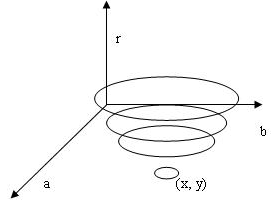
\includegraphics[width=1.1\linewidth]{yuan1.png} 
        \end{minipage}
        \quad
        \begin{minipage}[t]{0.4\linewidth}
            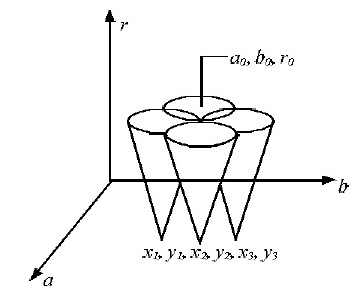
\includegraphics[width=1\linewidth]{yuan2.png} 
        \end{minipage}
    \end{figure}
    \begin{displaymath}
        (a-x_{i})^{2}+(b-y_{i})^{2}=r
    \end{displaymath}
\end{frame}

\begin{frame}
  \vspace{2cm}
  \centering
  \color{blue}\Huge{Thanks!}
  \vspace{1.5cm}
 

\end{frame}
%===============================================================================


\end{document}
